\newpage
\subsection{Arquitectura de la aplicación web}

La aplicación web fungirá como el panel de control central (\textit{dashboard}) del sistema. Estará dirigida a los administradores, investigadores y tomadores de decisiones, permitiéndoles visualizar el historial de detecciones, analizar el estado fitosanitario del bosque y gestionar los registros recolectados por los dispositivos móviles en campo.

\subsubsection{Arquitectura del Frontend (SPA)}

El desarrollo del \textit{frontend} se llevará a cabo utilizando el \textit{framework} \textbf{Angular}, adoptando el paradigma de \textit{Single Page Application} (SPA). Esta arquitectura garantizará una experiencia de usuario fluida, ya que la aplicación cargará una única página HTML y actualizará dinámicamente sus vistas sin necesidad de recargar el navegador en cada interacción.

La interfaz de usuario se construirá de manera modular utilizando \textbf{Angular Material}, una biblioteca de componentes de UI que implementa los lineamientos de \textit{Material Design}. Esto asegurará consistencia visual, accesibilidad nativa y un diseño responsivo que se adaptará automáticamente a diferentes resoluciones de pantalla (escritorio y tabletas). 

\subsubsection{Distribución estática y alojamiento seguro}

Aprovechando la naturaleza de la SPA, la aplicación web no requerirá un servidor de aplicaciones tradicional para su alojamiento. En su lugar, el código fuente de Angular se compilará en un conjunto de archivos estáticos (HTML, CSS y JavaScript) que se almacenarán en un \textit{bucket} de \textbf{Amazon S3} configurado exclusivamente para alojamiento estático.

Para garantizar una entrega rápida y segura del contenido a los usuarios, se desplegará \textbf{Amazon CloudFront} como Red de Entrega de Contenido (CDN). CloudFront almacenará en caché los artefactos estáticos en sus nodos perimetrales globales, reduciendo drásticamente la latencia de carga. Además, CloudFront se integrará con \textbf{AWS Certificate Manager (ACM)} para adjuntar un certificado SSL/TLS válido, forzando que todo el tráfico hacia la plataforma web viaje encriptado bajo el protocolo HTTPS.

\subsubsection{Consumo de API y visualización de datos}

La comunicación entre la aplicación web y el \textit{backend} \textit{serverless} se gestionará a través del módulo \textbf{HttpClient} nativo de Angular. Los servicios del \textit{frontend} realizarán peticiones asíncronas hacia los \textit{endpoints} expuestos en Amazon API Gateway para recuperar la información consolidada en la base de datos PostgreSQL y las imágenes almacenadas en S3.

Dado que el objetivo principal de la plataforma web es el análisis de resultados, se integrará la biblioteca \textbf{D3.js} (Data-Driven Documents). D3.js se utilizará para renderizar representaciones gráficas interactivas y complejas basadas en datos, tales como la distribución espacial de los árboles infectados, gráficas de series de tiempo sobre la propagación de insectos descortezadores y diagramas de calor. La manipulación directa del DOM que ofrece D3.js permitirá generar visualizaciones estadísticas altamente personalizadas que no serían posibles con bibliotecas de gráficos genéricas.

\subsubsection{Autenticación y seguridad en el cliente}

El acceso a la plataforma web estará estrictamente controlado mediante \textbf{Amazon Cognito}. El flujo de seguridad se implementará de la siguiente manera:

\begin{enumerate}
    \item \textbf{Inicio de sesión:} Los usuarios administradores se autenticarán ingresando sus credenciales en un formulario conectado al \textit{User Pool} de Cognito.
    \item \textbf{Gestión de Tokens:} Tras una autenticación exitosa, Cognito devolverá tokens de seguridad (ID Token y Access Token) basados en el estándar JWT. Estos tokens se almacenarán de forma segura en el navegador del cliente.
    \item \textbf{Interceptores HTTP:} Se configurará un \textit{HttpInterceptor} en Angular que capturará todas las peticiones salientes hacia el API Gateway y adjuntará automáticamente el \textit{Access Token} en la cabecera \texttt{Authorization}.
    \item \textbf{Protección de rutas (\textit{Guards}):} A nivel de navegación, se implementarán \textit{Route Guards} de Angular (\texttt{CanActivate}) para verificar la validez del token local antes de permitir el acceso a las vistas administrativas. Si un usuario no está autenticado o su sesión ha expirado, será redirigido inmediatamente a la pantalla de \textit{login}.
\end{enumerate}

\begin{figure}[H]
    \centering
     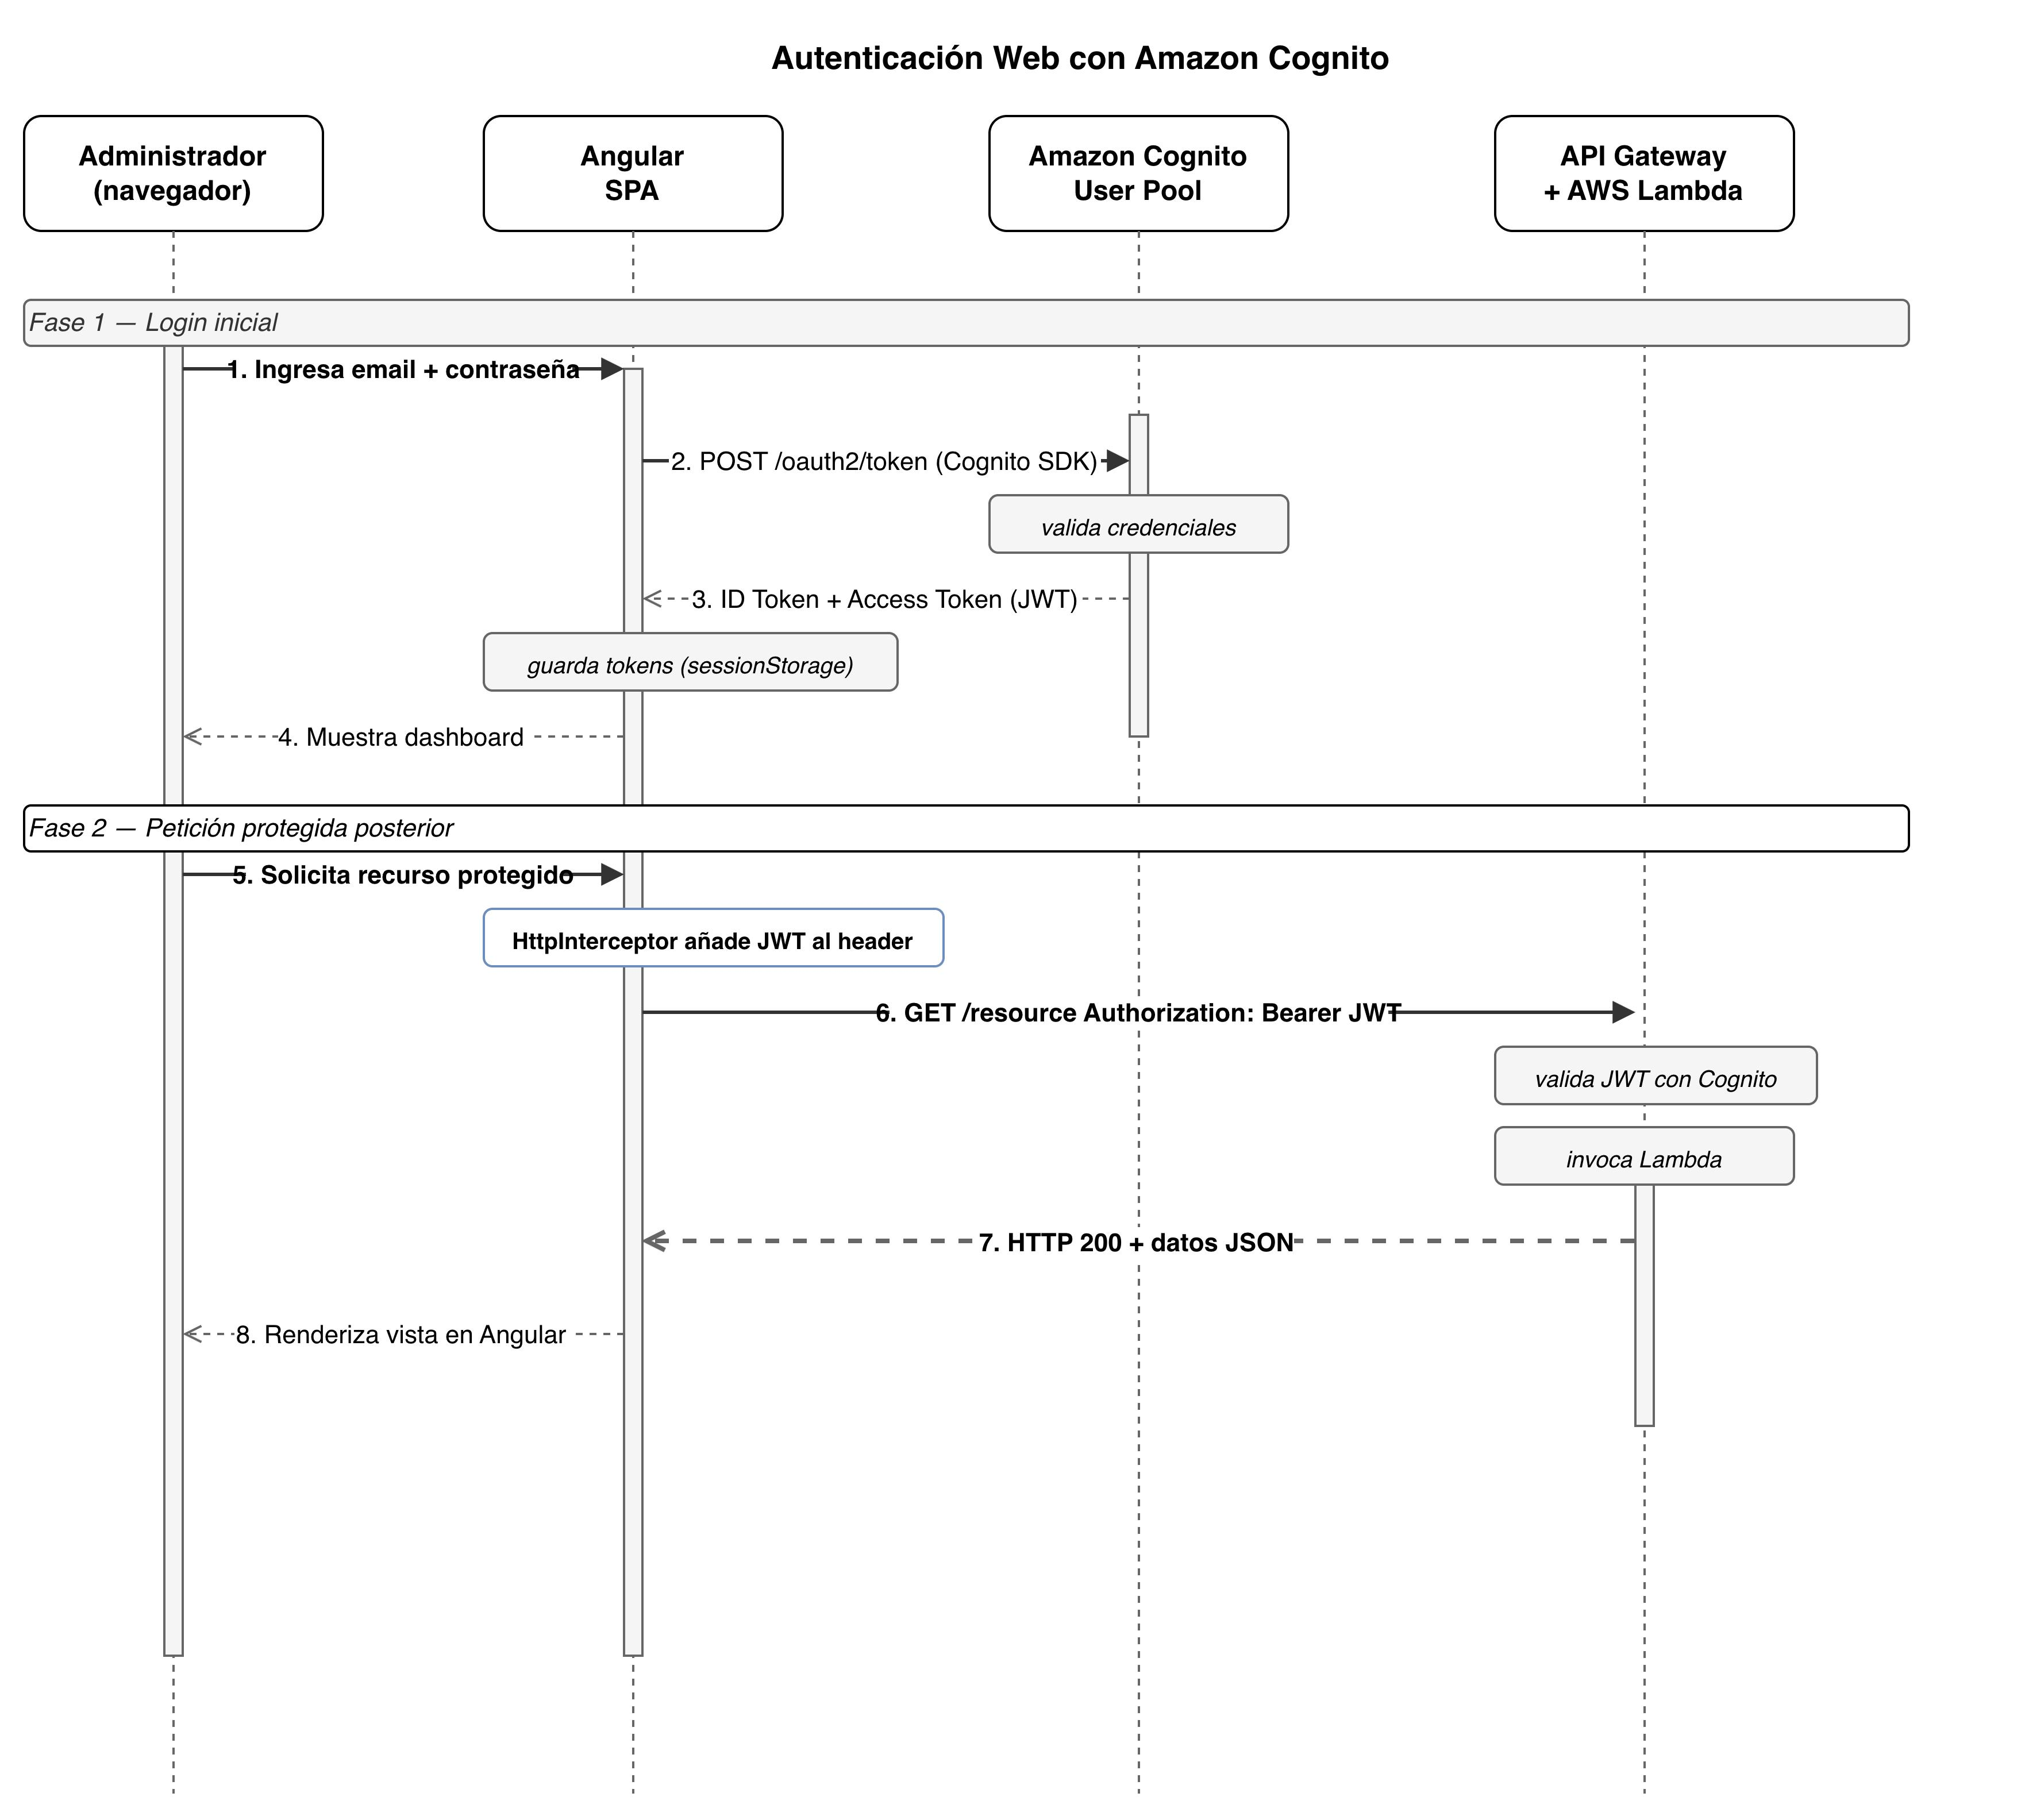
\includegraphics[width=0.95\textwidth]{images/C8/auth_web.jpeg}
    \caption{Flujo de autenticación y consumo seguro de API en la aplicación web.}
    \label{fig:flujo-autenticacion-web}
\end{figure}